\section{Overview of ATHLET and NuT software}


\subsection{ATHLET}
\ifSpeech
%%%%%%%%%%%%%%%%%%%%%%%%%%%%%%%%%%%%%%%%%%%%%%%%%%%%%%%%%%
\begin{frame}[t]{3: Overview of ATHLET and NuT software}
  \justifying
  
  \begin{itemize}
    \setlength\itemsep{0.5cm}
      \item ATHLET is a thermal-hydraulic system simulation code
      
      \item developed for the analysis of the \textbf{whole spectrum} of \textbf{operational conditions}
      
      \item for nuclear energy facilities
      
    \item The code provides specific models and methods for the \textbf{simulation of many types of nuclear power plants} 
        \begin{itemize}
             \setlength\itemsep{0.5cm}
            \item including \textbf{current Light Water Reactors}
            \item and \textbf{advance 3rd and 4th generations}
        \end{itemize}
    
  \end{itemize}

\end{frame}

%%%%%%%%%%%%%%%%%%%%%%%%%%%%%%%%%%%%%%%%%%%%%%%%%%%%%%%%%%
\begin{frame}[t]{4: Mathematical Model: before equations}
    \justifying
    
    \begin{itemize}
        \setlength\itemsep{0.5cm}
    
        \item \textbf{Physical processes} inside of \textbf{hydraulic circuits} of light-water reactors
        
        \item can be naturally described by a \textbf{two-phase thermo-fluiddynamic model}
        
        \item  based on conservation equations of mass, momentum and energy for liquid and vapor.
    \end{itemize}

\end{frame}
\fi


%%%%%%%%%%%%%%%%%%%%%%%%%%%%%%%%%%%%%%%%%%%%%%%%%%%%%%%%%%
\ifPresentation
\begin{frame}[t]{Mathematical Model}
    \spc
    \justifying
    \small
    
1. Liquid mass
\begin{equation} \label{eq:athlet-1}
\frac{\partial ((1-\alpha)\rho_{l})}{\partial t} + \nabla ((1-\alpha) \rho_{l} \vec{w_{l}}) = - \psi
\end{equation}


2. Vapor mass
\begin{equation} \label{eq:athlet-2}
\frac{\partial (\alpha \rho_{v})}{\partial t} + \nabla (\alpha \rho_{v} \vec{w_{v}}) = \psi
\end{equation}


3. Liquid momentum
\begin{equation} \label{eq:athlet-3}
\frac{\partial ((1-\alpha) \rho_{l} \vec{w_{l}})}{\partial t} + \nabla ((1-\alpha) \rho_{l} \vec{w_{l}} \vec{w_{l}}) + \nabla ((1 - \alpha)p) = \vec{F_{l}}
\end{equation}

4. Vapor momentum
\begin{equation} \label{eq:athlet-4}
\frac{\partial (\alpha \rho_{v} \vec{w_{v}})}{\partial t} + \nabla (\alpha \rho_{v} \vec{w_{v}} \vec{w_{v}}) + \nabla (\alpha p) = \vec{F_{v}}
\end{equation}

    \normalsize
\end{frame}


\begin{frame}[t]{Mathematical Model}
    \spc
    \justifying
    \small
5. Liquid energy
\begin{equation} \label{eq:athlet-5}
\frac{\partial \Big[ (1-\alpha)\rho_{l}(h_{l} + \frac{1}{2} \vec{w_{l}} \vec{w_{l}} - \frac{p}{\rho_{l}}) \Big]}{\partial t} + \nabla \Big[ (1-\alpha)\rho_{l}\vec{w_{l}}(h_{l} + \frac{1}{2} \vec{w_{l}} \vec{w_{l}}) \Big] = - p \frac{\partial (1 - \alpha)}{\partial t} + E_{l}
\end{equation}


6. Vapor energy
\begin{equation} \label{eq:athlet-6}
\frac{\partial \Big[ \alpha \rho_{v}(h_{v} + \frac{1}{2} \vec{w_{v}} \vec{w_{v}} - \frac{p}{\rho_{v}}) \Big]}{\partial t} + \nabla \Big[ \alpha\rho_{v}\vec{w_{v}}(h_{v} + \frac{1}{2} \vec{w_{v}} \vec{w_{v}}) \Big] = - p \frac{\partial \alpha}{\partial t} + E_{v}
\end{equation}

7. Volume vapor fraction
\begin{equation} \label{eq:athlet-7}
	\alpha = \frac{V_{v}}{V}
\end{equation}

    \normalsize
    \spc
    \textit{According to \cite{lt:ATHLMaM}}\\
\end{frame}


%%%%%%%%%%%%%%%%%%%%%%%%%%%%%%%%%%%%%%%%%%%%%%%%%%%%%%%%%%
\begin{frame}[t]{Mathematical Model: from PDEs to ODEs}

    \begin{columns}
        \column{0.47\textwidth}
            \begin{figure}[htpb]
                \centering
                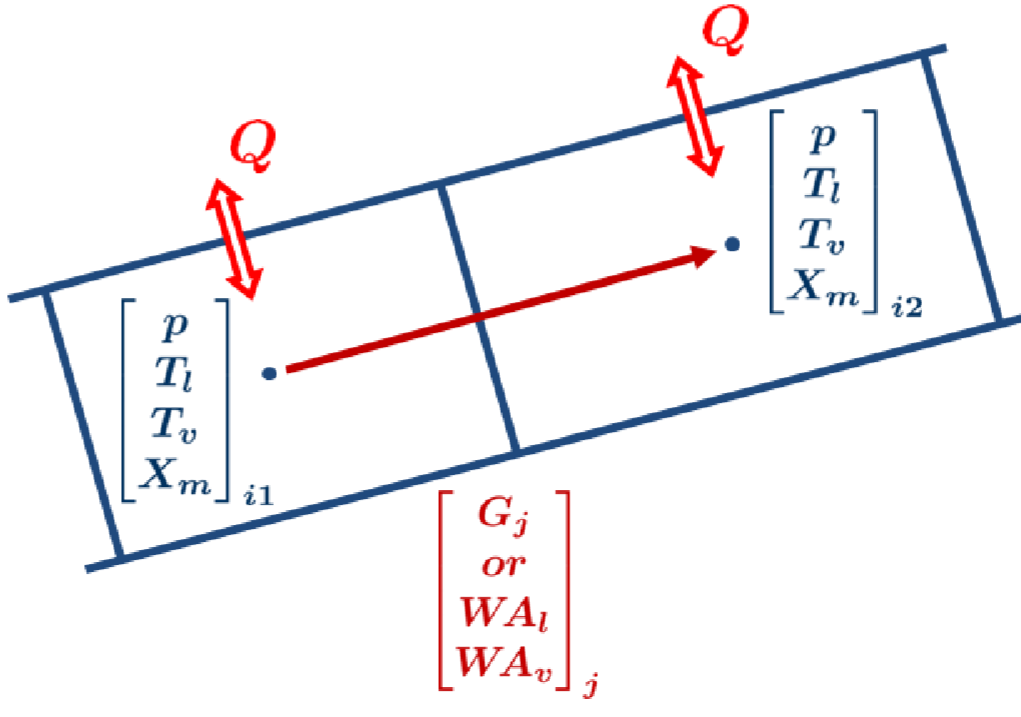
\includegraphics[width=0.8\textwidth]{figures/introduction-1d-fvm.png}
                \caption{ATHLET: one dimensional \textbf{Finite Volume} formulation of the problem \cite{tims-presentation}}
                \label{fig:introduction-1d-fvm}
            \end{figure}
        
        
        \column{0.5\textwidth}
        \justifying
        The system is transformed to a non-autonomous system of \textbf{ordinary differential equations} and expressed as an \textbf{initial value problem} after spatial finite-volume integration and some mathematical transformations \cite{lt:ATHLMaM}.
        
        
        \small
        \begin{equation} \label{eq:athlet-8}
	        \frac{dy}{dt} = f(t,y), \;  t_{0} \leq t \leq t_{F} \; y(t_{0}) = y_{0}
        \end{equation}
        \normalsize

        where $y \in \mathbb{R}^{N}$ is a composite vector of variables, $f$ is a non-linear function such that $f : \mathbb{R} \times \mathbb{R}^{N} \supset \Omega  \rightarrow \mathbb{R}^{N}$  .\\

    \end{columns}

\end{frame}

\fi

\ifSpeech
%%%%%%%%%%%%%%%%%%%%%%%%%%%%%%%%%%%%%%%%%%%%%%%%%%%%%%%%%%
\begin{frame}[t]{6: Mathematical Model: after equations}
    \justifying
    
    \begin{itemize}
        \setlength\itemsep{0.5cm}
    
        \item The system is \textbf{transformed} to a \textbf{non-autonomous} system of ODEs
        
        \item \textbf{expressed} as an \textbf{initial value problem}
        
        \item  After 
        
        \begin{itemize}
            \item Spatial Finite-Volume Integration
            
            \item some \textbf{advanced mathematical transformations}
        \end{itemize}
        
    \end{itemize}

\end{frame}

%%%%%%%%%%%%%%%%%%%%%%%%%%%%%%%%%%%%%%%%%%%%%%%%%%%%%%%%%%
\begin{frame}[t]{7-1: Numerical Integration: 6-stage W-method
}
    \justifying

    \begin{itemize}
        \setlength\itemsep{0.5cm}
        
        \item Analysis of the system shows the problem is stiff 
        
        \item hence, must to be solved with an implicit solver
        
        \item ATHLET uses a \textbf{6-stage W-method}
        
        \item which \textbf{belongs} to the \textbf{family of Linearly Implicit Method} 
        
        \item in particular \textbf{Rosenbrock methods}
        
        \item the method can be viewed as following
    \end{itemize}
    
\end{frame}



\begin{frame}[t]{7-2: Numerical Integration: 6-stage W-method}

    \justifying
  

        \begin{itemize}
            \setlength\itemsep{0.5cm}
            \item \textbf{Number} of stages determines the \textbf{oder} of the method
            \item Each stage is solved via \textbf{Implicit Euler method}
            \item Only \textbf{one Newton's} iteration is used for Imolicit Euler step 
            \item In contrast to the Rosenbrock methods, W-methods uses a \textbf{Jacobian matrix approximation}
        \end{itemize}

    \normalsize
\end{frame}

\fi


%%%%%%%%%%%%%%%%%%%%%%%%%%%%%%%%%%%%%%%%%%%%%%%%%%%%%%%%%%
\ifPresentation
\begin{frame}[t]{Numerical Integration: 6-stage W-method}
    \justifying
    
    \begin{equation}
        (I - h_{i}J)\delta y_{ij} = h_{i} f(t_{0} + j \cdot h_{i}, y_{0} + \sum^{j-1}_{l = 0} \delta y_{il}) + h^{2} \frac{\partial f_{0}}{\partial t}
    \end{equation}
    
    where $j=0, \dots, i - 1$; $h_{i} = h / i$; $i = 1, 2, 3$

    \begin{figure}[htpb]
          \centering
          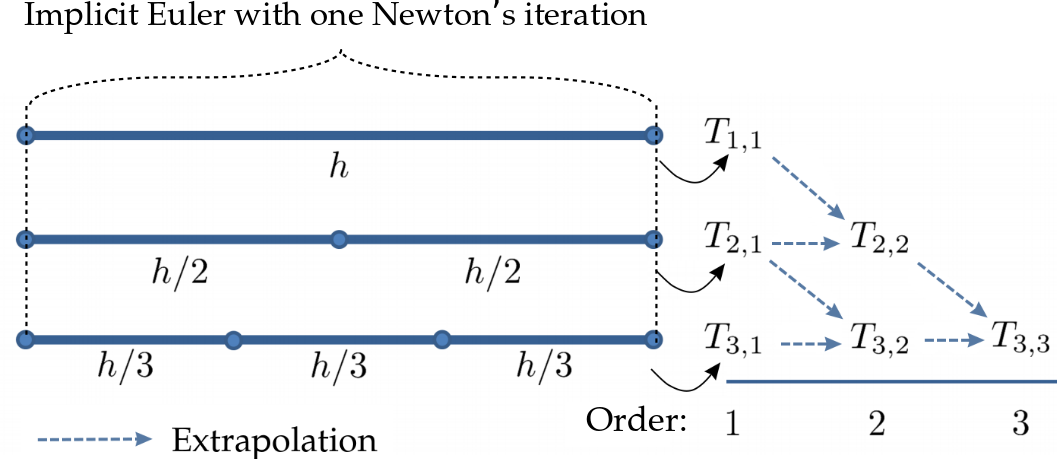
\includegraphics[width=0.8\textwidth]{figures/introduction-rosenbrock-scheme.png}
        \caption{A general view on 6-stage W-method \cite{tims-presentation}}
        \label{fig:introduction-w-method-scheme}
    \end{figure}

\end{frame}

\fi
